% Figure~\ref{fig:ML_assisted_process}
% (Section 4, Phase 2: ML-assisted measurement process).
%
% Replaces ML_assisted_process.jpg, a drawing taken from an IEEE I&M Society
% course slide (S. Shirmohammadi, "Quantifying Uncertainty in Machine
% Learning-Assisted Measurements"). Same flow, redrawn in the notation of the
% paper: measurement -> dataset -> trained model \hat f (estimate of f) ->
% indirect measurement \hat y = \hat f(x); the input quantities measured at
% inference are added, so that the two uncertainty groups connect to
% u_physical and u_model of Figure 3.
%
% Compiles with plain pdflatex to a tightly-cropped vector PDF.
% Okabe-Ito colours as in Figure 3: bluish green = data / input quantities,
% reddish purple = model.
\documentclass{article}
\usepackage{amsmath}
\usepackage{amssymb}
\usepackage{tikz}
\usetikzlibrary{arrows.meta, positioning, calc, shapes.geometric, decorations.pathreplacing}

\definecolor{okGreen}{HTML}{009E73}
\definecolor{okPurple}{HTML}{CC79A7}

\pagestyle{empty}
\hyphenpenalty=10000
\exhyphenpenalty=10000
\newsavebox{\figbox}
\newlength{\figborder}
\setlength{\figborder}{4pt}

\newcommand{\vx}{\mathbf{x}}
\newcommand{\fhat}{\hat{f}}

\begin{document}
\begin{lrbox}{\figbox}%
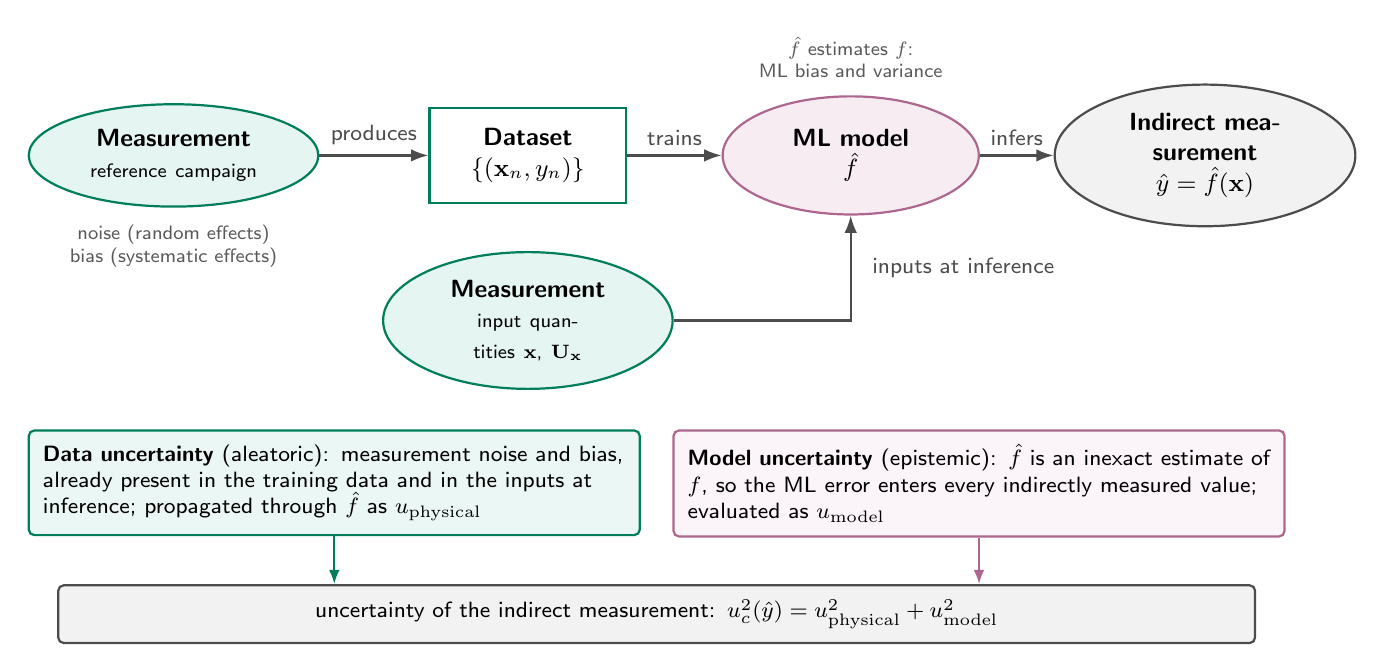
\begin{tikzpicture}[
  font=\sffamily\footnotesize,
  meas/.style={ellipse, draw=okGreen!80!black, thick, fill=okGreen!10,
    text width=24mm, align=center, inner sep=1mm, minimum height=13mm, font=\sffamily\small},
  data/.style={rectangle, draw=okGreen!80!black, thick, fill=white,
    text width=22mm, align=center, inner sep=1.5mm, minimum height=12mm, font=\sffamily\small},
  model/.style={ellipse, draw=okPurple!85!black, thick, fill=okPurple!14,
    text width=21mm, align=center, inner sep=1mm, minimum height=15mm, font=\sffamily\small},
  result/.style={ellipse, draw=black!70, thick, fill=black!5,
    text width=25mm, align=center, inner sep=1mm, minimum height=13mm, font=\sffamily\small},
  arrow/.style={-{Latex[length=2.2mm,width=1.6mm]}, thick, draw=black!70},
  albl/.style={font=\sffamily\footnotesize, text=black!70, above},
  note/.style={font=\sffamily\scriptsize, text=black!65, align=center},
  group/.style={rectangle, rounded corners=2pt, thick, align=left, inner sep=1.8mm,
    font=\sffamily\footnotesize},
]
% ---------------- training chain ----------------
\node[meas]   (m)  at (0,0)    {\textbf{Measurement}\\{\scriptsize reference campaign}};
\node[data]   (d)  at (4.5,0)  {\textbf{Dataset}\\$\{(\vx_n, y_n)\}$};
\node[model]  (f)  at (8.6,0)  {\textbf{ML model}\\$\fhat$};
\node[result] (y)  at (13.1,0) {\textbf{Indirect measurement}\\\mbox{$\hat y = \fhat(\vx)$}};

\draw[arrow] (m) -- node[albl]{produces} (d);
\draw[arrow] (d) -- node[albl]{trains} (f);
\draw[arrow] (f) -- node[albl]{infers} (y);

% annotations under the chain
\node[note, anchor=north] at ($(m.south)+(0,-1mm)$)
  {noise (random effects)\\bias (systematic effects)};
\node[note, anchor=south] at ($(f.north)+(0,1mm)$)
  {$\fhat$ estimates $f$:\\ML bias and variance};

% ---------------- inputs at inference ----------------
\node[meas, anchor=north] (mx) at ($(d.south)+(0,-6mm)$)
  {\textbf{Measurement}\\{\scriptsize input quantities $\vx$, $\mathbf{U}_{\vx}$}};
\draw[arrow] (mx.east) -| (f.south);
\node[font=\sffamily\footnotesize, text=black!70, anchor=west]
  at ($(f.south |- mx.east)!0.5!(f.south)+(1.5mm,0)$) {inputs at inference};

% ---------------- uncertainty groups ----------------
\node[group, draw=okGreen!80!black, fill=okGreen!8, anchor=north west, text width=74mm]
  (gD) at ($(m.west |- mx.south)+(0,-5mm)$)
  {\textbf{Data uncertainty} (aleatoric): measurement noise and bias, already
   present in the training data and in the inputs at inference; propagated
   through $\fhat$ as $u_{\mathrm{physical}}$};
\node[group, draw=okPurple!85!black, fill=okPurple!8, anchor=north west, text width=74mm]
  (gM) at ($(gD.north east)+(4mm,0)$)
  {\textbf{Model uncertainty} (epistemic): $\fhat$ is an inexact estimate
   of $f$, so the ML error enters every indirectly measured value; evaluated
   as $u_{\mathrm{model}}$};

% combined result
\node[rectangle, rounded corners=2pt, draw=black!70, thick, fill=black!5, anchor=north,
      minimum width=152mm, inner sep=1.8mm, font=\sffamily\footnotesize] (uc)
  at ($(gD.south east)!0.5!(gM.south west)+(0,-6mm)$)
  {uncertainty of the indirect measurement:\enspace
   \mbox{$u_c^2(\hat y) = u_{\mathrm{physical}}^2 + u_{\mathrm{model}}^2$}};
\draw[thick, okGreen!80!black, -{Latex[length=1.8mm]}] (gD.south) -- (gD.south |- uc.north);
\draw[thick, okPurple!85!black, -{Latex[length=1.8mm]}] (gM.south) -- (gM.south |- uc.north);

\end{tikzpicture}%
\end{lrbox}%
% crop the page to the picture
\pdfpagewidth=\dimexpr\wd\figbox+2\figborder\relax
\pdfpageheight=\dimexpr\ht\figbox+\dp\figbox+2\figborder\relax
\pdfhorigin=\figborder
\pdfvorigin=\figborder
\shipout\hbox{\usebox{\figbox}}
\end{document}
